% \chapter{THE STANDARD MODEL OF PARTICLE PHYSICS}
\chapter{ALPHABET SOUP: H, SM, BEH, EWSB}
\label{ch:theory}

The Standard Model (SM) is a collection of the most accurate and self-consistent particle physics theories that mathematically describe the properties of particles within the universe and their interactions with each other.
For the past century, some of the most brilliant minds in physics have spent their entire careers to develop equations, mathematical tricks, and completely novel ideas to help build a solid foundation for the SM.
To demonstrate the unparalleled accuracy with which the SM predicts physical phenomena, one can compare the experimentally measured anomalous magnetic moment of the electron
\begin{equation*}
    a_e^{\mathrm{exp}} = 0.001\ 159\ 652\ 180\ 73(28)
\end{equation*}
to the value predicted by the SM
\begin{equation*}
    a_e^{\mathrm{pred}} = 0.001\ 159\ 652\ 181\ 643(764).
\end{equation*}
An impressive agreement to better than one part per trillion.

On the other hand, the SM has no explanation for some observed physical phenomena (Sec.~\ref{sec:shortcomings}), \eg the existence of dark matter~\cite{particle_data_group_review_2020}, and is thus not a fully descriptive model of the Universe.
Furthermore, the Collider Detector at Fermilab (CDF) Collaboration recently measured the mass of the \PW boson to be $80\,433.5 \pm 9.4\MeV$, whereas the SM expectation $80\,357 \pm 4\MeV$---a discrepancy of 7.0 standard deviations~\cite{cdf_collaboration_high-precision_2022}---as is shown in Fig.~\ref{fig:wmass}.
Recent results from the Baksan Experiment on Sterile Transitions suggest electron neutrinos oscillating between sterile neutrino states~\cite{PhysRevLett.128.232501}.
Nevertheless, the SM has laid important foundations in particle physics for over 100 years and is fully explained with the discovery of the Higgs boson in 2012 TODO:CITE.
%%%%%%%%%%%%%%%%%%%%
\begin{figure}[pbth]
    \centering
    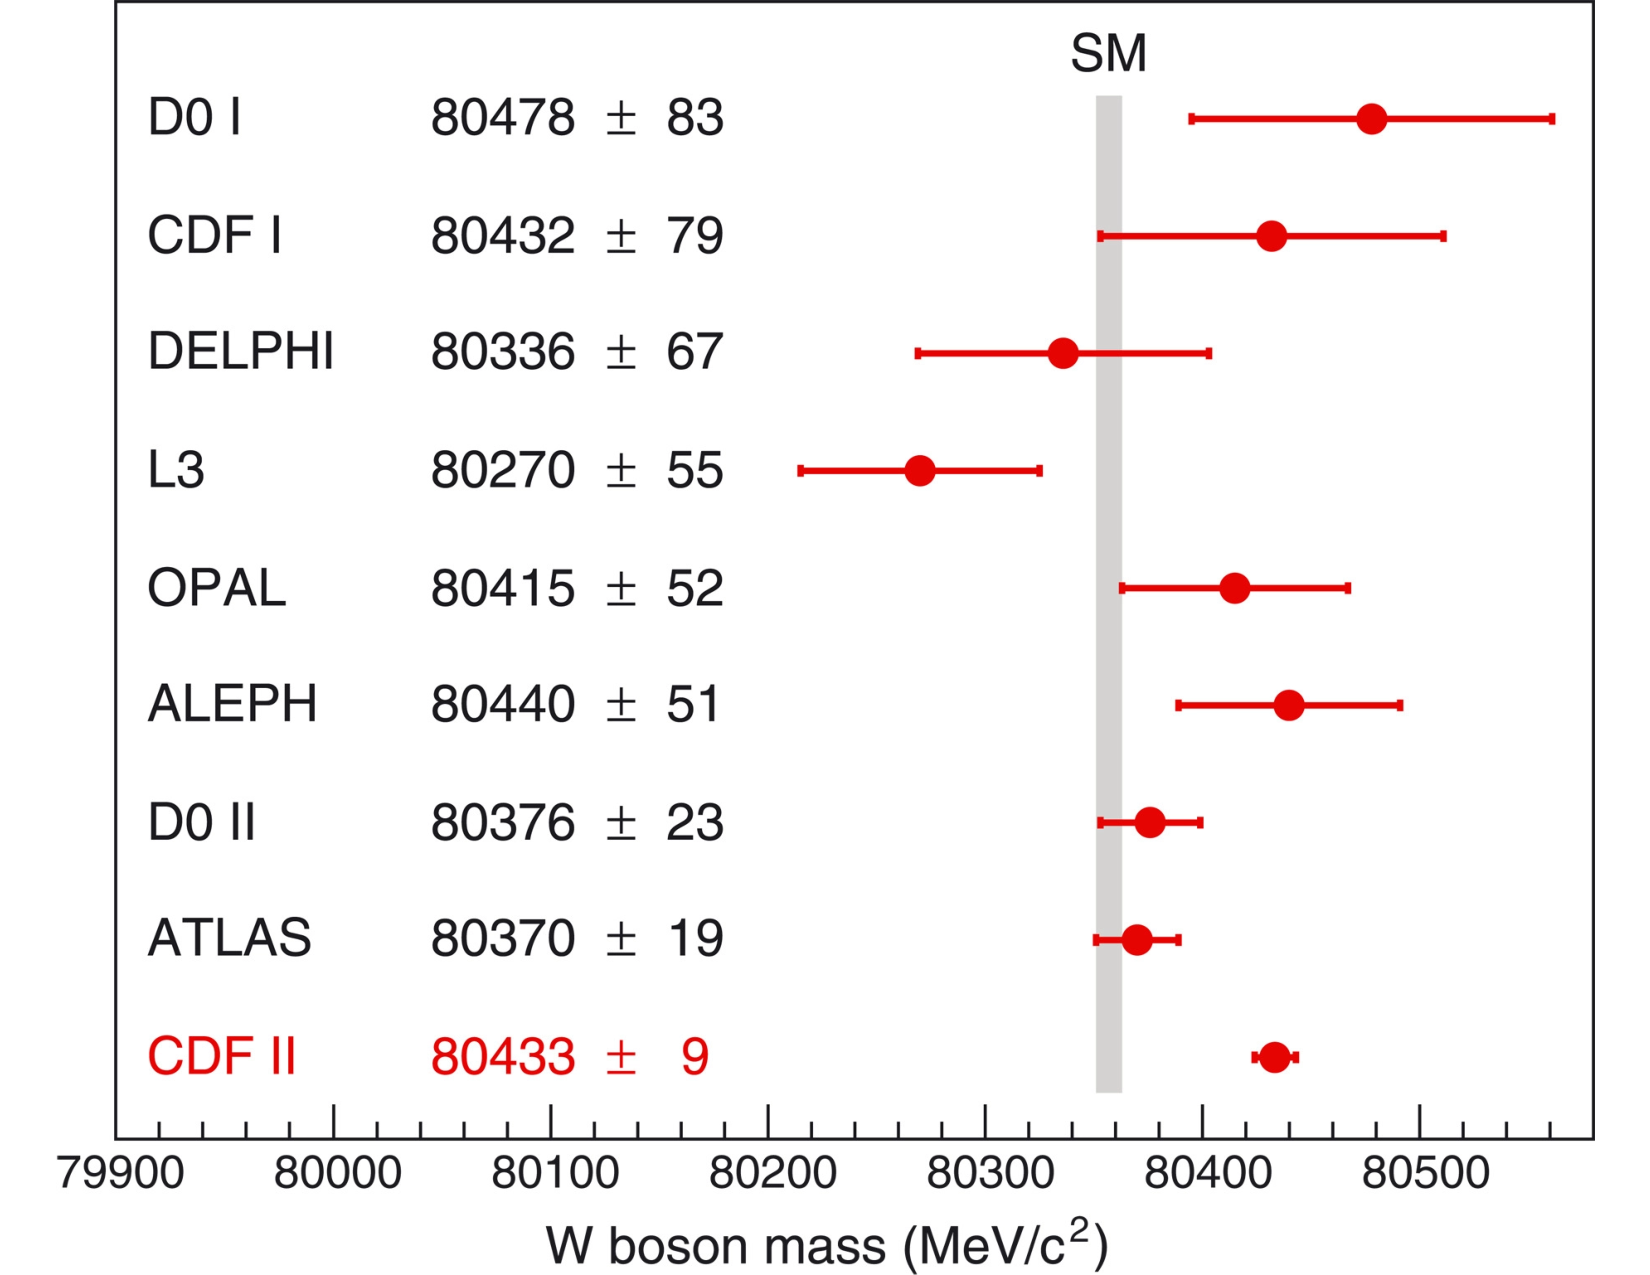
\includegraphics[height=5cm,keepaspectratio]{figures/sm/wmass.pdf}
        \caption{Precision measurements of the W-boson mass performed by various collaborations.} 
        \label{fig:wmass}
    \end{figure}
    %%%%%%%%%%%%%%%%%%%%
% CDF MW=80,433.5 +- 6.4 stat +- 6.9 syst = 80,433.5 +- 9.4 MeV/c2
% SM expectation: MW=80,357 +- 4inputs +- 4theory MeV

The remainder of this chapter presents a general overview (Sec.~\ref{sec:sm_overview}) of the particles and forces described by the SM, followed by a brief analysis of the mathematical underpinnings of the SM (Sec.~\ref{sec:sm_math}), and then finally a brief description of the shortcomings of the SM (Sec.~\ref{sec:shortcomings}).
%and finally a summary of the physics of the Higgs boson, which is integral to this dissertation.

% First, the major players that make up the SM---the fundamental particles---are introduced.
% Next, an explanation is given on how the infamous Higgs boson completed the SM.
% Finally, problems of the SM are described and how its claims can be tested.
% Some of the most brilliant minds in physics have worked for their entire careers to develop equations and  novel ideas solutions to problems which perplexed mankind for more than 100 years a century's worth of work to  
% an impressively accurate 
% It is currently the most accurate model of particles and their interactions with each other - and frankly - it is {\it quite} impressive!

% Allow me to paint the picture, as I see it:
% We all are included in the Song of the Universe.
% This song is called "Reality" and this tune has been playing for nearly 13.8 billion years, or so the cosmologists tell us. 
% To me, the notes and lines on this music staff resemble particle physics.
% The staff lines are like field lines which permeate the Universe.
% I imagine them like the strings on a violin.
% When a field line is plucked, you a create a note: a particle.
% If you pluck an electromagnetic field line, you get a photon.
% If you pluck an electron field line, you get an electron.
% A Higgs field line, a Higgs boson.
% Particle Physicists are curious about these notes and strings, 
% the particles and the fields and how they interact with each other.

% So, how does the song go?

SM OF PARTICLE PHYSICS CHAPTER OUTLINE
OVERVIEW:
- Main concept:
- Everything is particles!
    Fields permeate all of space.
    Their mathematical treatment is handled in Sec.TODO.
    Particles are excitations of the fields.
    Interactions are between particles 
    Bosons
    Fermions
        Leptons
        Quarks
MATHEMATICAL FRAMEWORK
- Show SM Lagrangian.
- Derive interactions between particles.
    BEH MECHANISM
    - Robert Brout, François Englert, and Peter Higgs claimed that elementary particles acquire their masses via spontaneous EWSB. (reword!)
    - Sheldon Glashow, Abdus Salam, and Steven Weinberg were able to unify the weak and electromagnetic forces into a single force, above the unification energy of 246\GeV.
    - In 1973 the Gargamelle collaboration experimentally confirmed the existence of the electroweak force by discovering neutral currents in neutrino scattering experiments.
    - Furthermore, in 1983 the UA1 and UA2 collaborations used proton-antiproton collisions to discover the theorized \PW and \PZ electroweak gauge bosons.
SHORTCOMINGS OF THE SM
- Each of these is a new paragraph?:
- Neutrino oscillations confirm that neutrinos \emph{do} have masses but interaction with the Higgs field is not responsible for this origination.
- No gravity.
- Why matter and no antimatter?
- Where does dark matter fit in?
- Why should there be exactly 3 generations of fermions?
- Although the SM does not answer any of the above questions, 

\section{Overview}
\label{sec:sm_overview}

The SM is a renormalizable quantum field theory defined in terms of a Lagrangian tha describes interactions between fundamental particles as governed by the strong, weak, and electromagnetic forces. It is a non-Abelian gauge theory comprising interacting field theories based on gauge invariance constructed within the framework of quantum mechanics and special relativity. The SM exhibits invariance under the symmetry group

\begin{equation}
    \text{SU}(3)_C \times \text{SU}(2)_L \times \text{U}(1)_Y
\end{equation}

where SU(3)$_C$ invariance explains the existence of gluons ($g$) as the mediators of the strong force, described by quantum electrodynamics (QCD), and the $\text{SU}(2)_L \times \text{U}(1)_Y$ invariance results in the $W^\pm$, $Z^0$, and $\gamma$ bosons as mediators of the electroweak force, described by the unified electroweak theory and quantum electrodynamics. Interactions via the strong, electromagnetic, and weak forces are restricted to particles carrying a color charge, electric charge, and a weak charge, respectively. The SM formulation lacks the ability to describe gravity on a quantum level and might actually be incompatible with the most successful modern theories of gravitation. Gravitational effects are negligible at subnuclear scales.

% Weak hypercharge, weak isospin (L reminds us that this interaction only effects left-handed fermions), color charge
% \textit{Q: What is the difference between $U(1)_q and U(1)_Y$?}
% \textit{Q: Does L stand for left-handed?}

% All observers must Lagrangian 
% The connection between conservation laws and symmetries is best analyzed via Lagrangian mechanics.

% Each Lagrangian has its own set of ``Feynman rules''.

\textbf{The Particles: The Players on the Fields}

Contrary to intuition, fundamental particles are not hard, billiard-ball-like objects as is often perceived.
Instead the SM predicts that every particle is actually an \emph{excitation} of its corresponding field.
So for example the electron is an excitation of the \emph{electron field}, $\psi_{e}(x)$, a bispinor that describes a spin-1/2 field which follows the Dirac equation: 
% \begin{equation*}
%     (i\hbar c \gamma^{\mu}{\partial}_{\mu} 
%     - mc^{2})\psi(x) = 0.
% \end{equation*}
In fact, \emph{every} electron is an excitation of this same electron field. 
An electron is identical to every other electron in every way (same mass, same charge, etc.).
Quantum Mechanics (QM) does a fine job of describing how slow-moving particles behave.
However, as soon as particles begin moving at 30.5\% of the speed of light (91.4 $91.4 E6$ m/s), then there is a 5\% difference between the particle's rest mass energy ($E = mc^2$) and its total relativistic energy ($E = \gamma mc^2$).
In other words, fast-moving particles must account for effects due to Special Relativity (SR).
The merger of QM and SR gives rise to Quantum Field Theory (QFT) - the backbone of the SM.

Fig.~\ref{fig:particulartable} shows all the fundamental particles that have been discovered up to the present day.
The phrase ``fundamental particle'' just means that the particle is not composed of anything smaller than itself. 
These particles are not just diabolical creations from theorists. 
No, these particles are precisely defined, mathematical objects whose existence has been predicted by the SM and experimentally verified time and time again in the laboratory.
%%%%%%%%%%%%%%%%%%%%
\begin{figure}[pbth]
\centering
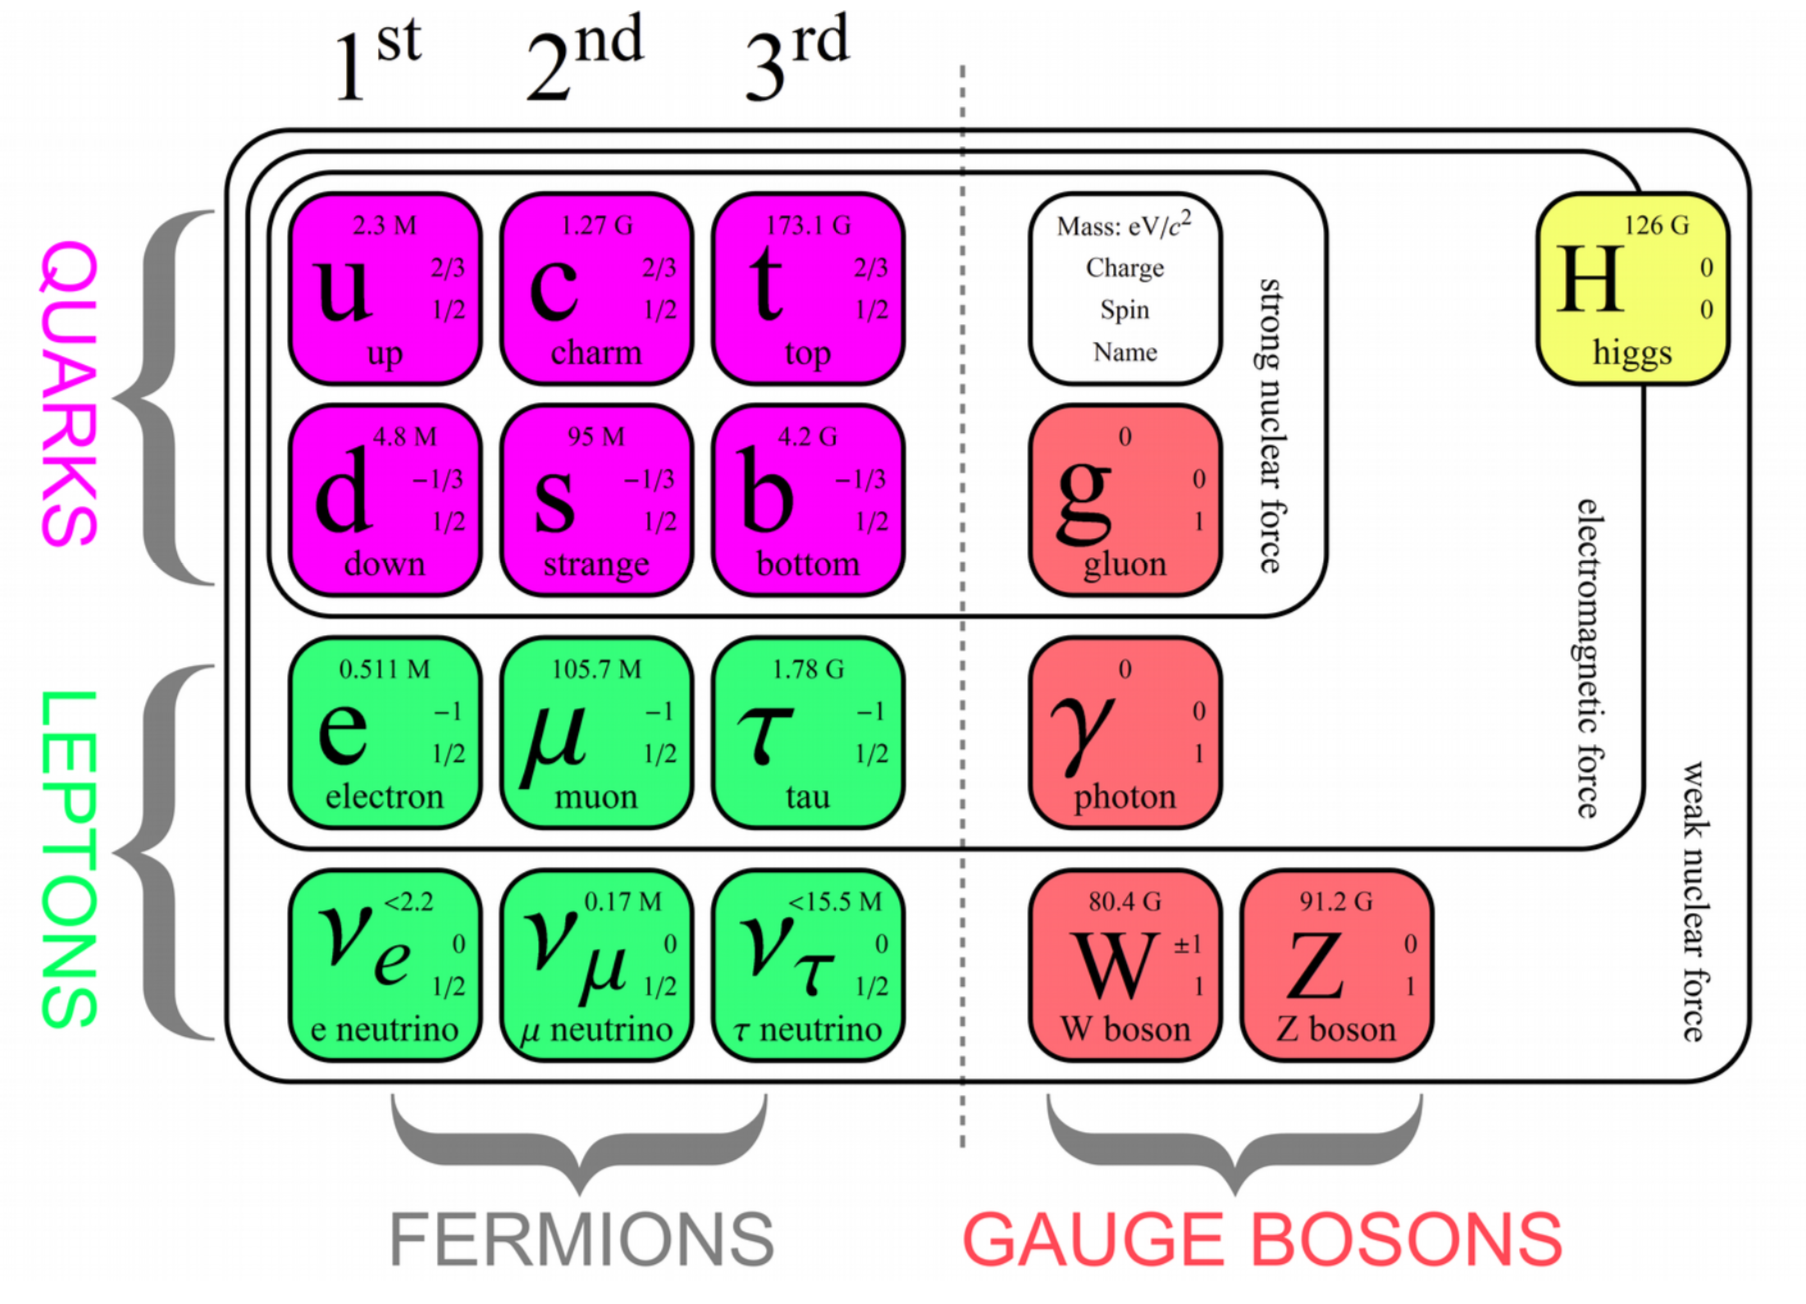
\includegraphics[width=15cm,height=15cm,keepaspectratio]{figures/sm/particular_table_updated.png}
    \caption{The fundamental particles of the Standard Model.} 
    \label{fig:particulartable}
\end{figure}
%%%%%%%%%%%%%%%%%%%%

Each particle has a unique set of properties (like mass, electric charge, spin, \etc.) that distinguish it from all the other particles. 
It is one of the primary goals of particle physics to determine these properties, because ultimately their properties determine their \emph{interactions} with one another. 

Without further ado, let's meet the particles.
There are two major types: \emph{bosons} and \emph{fermions}.
We are going to take a non-traditional route and introduce the bosons first, then the fermions.

\textbf{Bosons: Use the Force}

% The bosons are said to be the "force carrier" particles. 
% In particle physics, when two particles interact with one another, how do they do it? 
% instead an intermediate particle, very often a boson, is said to ``mediate'' the interaction and be the entity responsible which transfers the force from one particle to the other. 
Ever wonder how two electrons "know" that they are near each other and that they should repel? 
Fig.~\ref{fig:ee_scattering} shows a Feynman diagram of two electrons ``communicating'' with each other by means of an intermediate photon.
I like to think of it as the two electrons ``playing catch'' with the photon.
The first electron recoils from the throw and then the second electron recoils from catching the photon.
The photon carries some momentum away from the first electron and brings it to the second one, therefore making it look as if the two electrons are repelling one another!
The photon isn't \emph{real} of course - it is said to be a \emph{virtual} photon.
Now we see why bosons are called the force carriers.
%%%%%%%%%%%%%%%%%%%%
\begin{figure}[pbth]
\centering
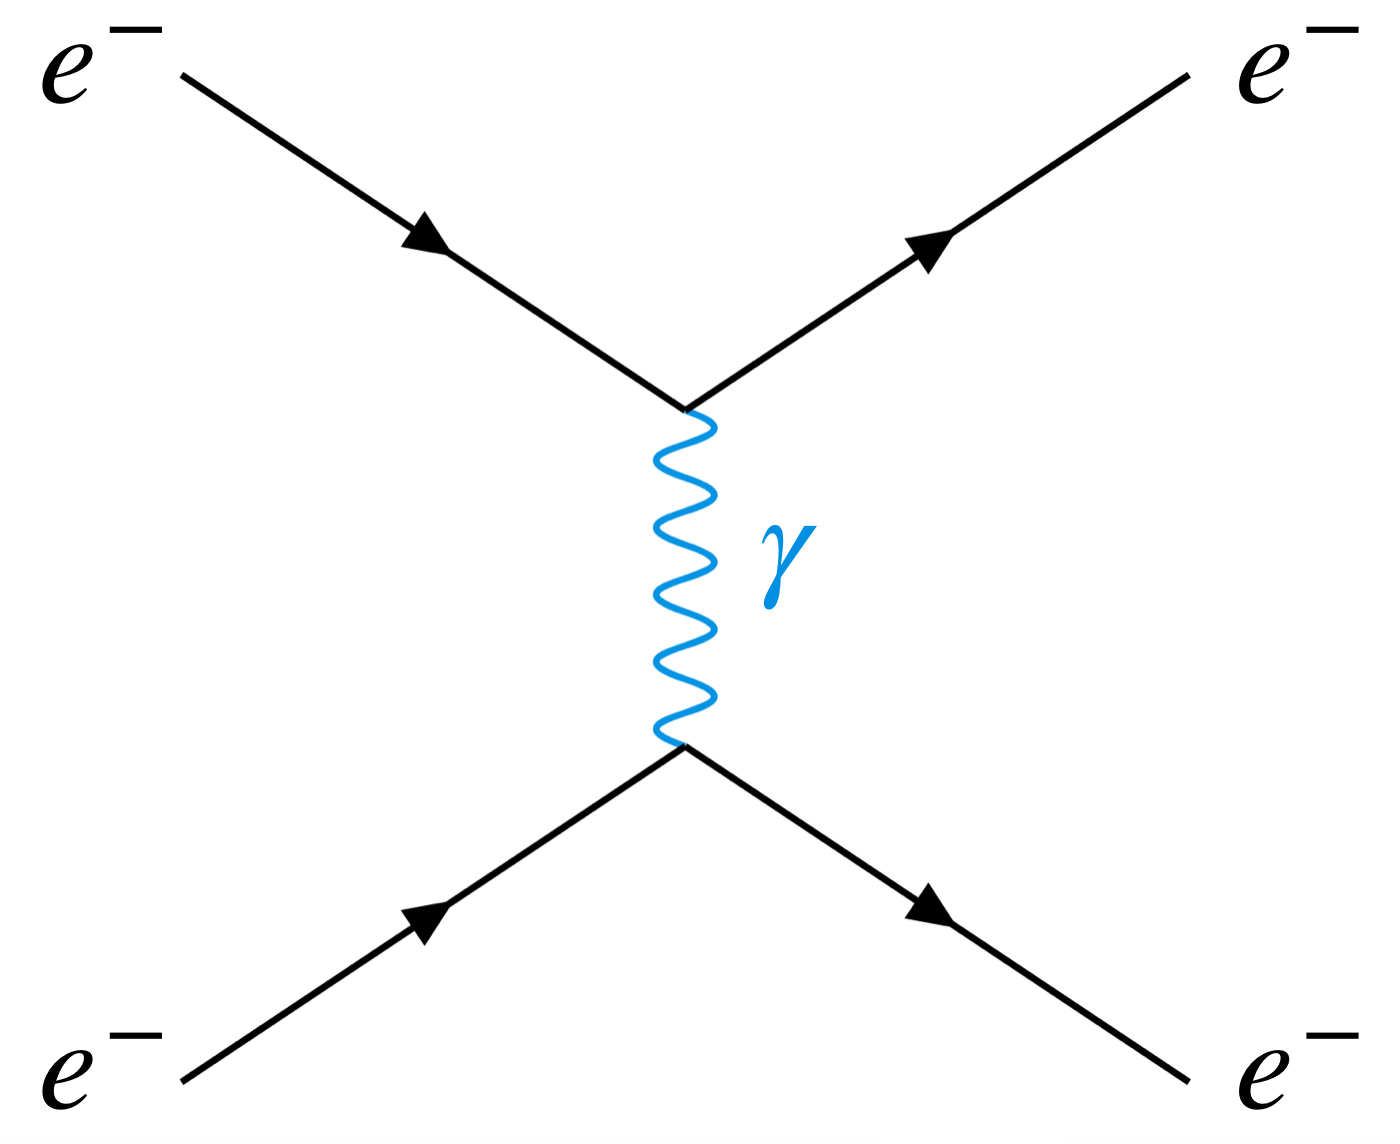
\includegraphics[width=6cm,height=6cm,keepaspectratio]{figures/sm/ee_scattering_moeller.png}
    \caption{A Feynman diagram showing electron-electron scattering, also known as Møller scattering.} 
    \label{fig:ee_scattering}
\end{figure}
%%%%%%%%%%%%%%%%%%%%

% Quantum Electrodynamics, one of the theories cooped up in the SM, is a quantum field theory that can mathematically describe one electron "throwing" a photon to the other.
A diagram such as the one above is a Feynman diagram and it gives us a wonderfully simple way to visualize particle physics processes.
It's not \emph{actually} what happens between the particles, but it is a good starting point.
Each diagram is actually a single, scalar number -
a complicated QFT integral that tells you how likely a process is to happen.
Another benefit to Feynman Diagrams is that they are kind of like tinker toys, 
in that you can string them together in novel ways to predict real-world processes.
Quantum Electrodynamics (QED), one of the theories that make up the SM, mathematically describes and predicts the electrons mediating such a photon between them. 
It's not just limited to electrons mediating photons, however.
QED and other QFTs can predict to astounding accuracy how likely a process is to happen, between whichever particles and fields. 
You just need to know their properties first.
% \emph{Any} particle with electric charge can interact via the electromagnetic force (EM) force.

We have now met the first force carrier: the photon.
It is a massless particle and is the mediator of the EM force. 
Photons only interact with particles that carry \emph{electric charge}.
Depending on what kind of charge a particle carries, determines with which bosons it may interact and via which forces.
Speaking of forces, the four fundamental forces found in nature, along with their decreasing, relative strength are: 
% (1) strong, (2) EM, (3) weak, (4) gravitational
\begin{enumerate}
    \item strong force $(1)$
    \item EM force $(10^{-1})$
    \item weak force $(10^{-6})$
    \item gravitational force $(10^{-40})$
\end{enumerate}
If the photon is the mediator of the EM force, then what mediates the other forces?

The mediators of the strong force are the 8 {\bf gluons}. 
Similar to the photon, they are also massless, but that's about all they have in common. 
Gluons are trapped inside of protons, neutrons, and other hadronic matter. 
They are responsible for ``glueing'' nuclei to together, hence their name.
Just as photons can only interact with particles that have electric charge, gluons can only interact with particles that have \emph{color} charge.
Interestingly, gluons themselves carry color charge which they mediate back and forth between quarks (fermions discussed below).
This is quite different from the photon which itself does not carry electric charge. 
There are three kinds of color charges: red, green, and blue.
Every gluon carries two color charges:
one kind of color and an anticolor: antired, antigreen, or antiblue.

There are three bosons which mediate the weak force: the Z, W$^+$, and W$^-$.
They are extraordinarily massive particles, weighing in at 91.2 GeV for the Z and 80.4 GeV for both kinds of W bosons. 
That means the W bosons weigh more than an iron atom! These bosons interact with any particle that carries ``weak hypercharge''.
The weak force has plagued physicists for nearly a century until only recently.
Particles which decay via the weak force live an astonishingly long time. 
Take for example the neutral pion ($\pi^0$). 
It decays very quickly, via the EM force, into two photons on the order of $10^{-18}$ s.
Now take the charged Kaon ${\rm K^+}$. 
This particle decays into three charged pions, but takes on average $10^{-8}$ s to do so.
Over 10 orders of magnitude different from the pion decay.
This is because the charged kaon decays via the weak force.

The last boson not yet mentioned is the scalar Higgs boson, which is introduced in Sec.TODO below.

% 1. There are 12 kinds fermions which are the matter particles and comprise all the matter that you see and feel
% 2. And in the other group there are 5 kinds of bosons, which are the force carriers and help fermions communicate with each other. 

\textbf{Fermions: Each One Matters}
There are 12 kinds of fermions - the matter particles of the Universe. 
They comprise all the ``stuff'' that we see and feel.
All fermions have half-integer spin, typically a value of 1/2. 
The fermions can be split into two groups depending on if they interact with the strong force (quarks) or not (leptons).
Let's consider the leptons first.

{\bf Leptons:}
% Ultimately all the matter we see, feel, and interact with daily is composed of fermions.
% Referring back to Fig.~\ref{fig:particulartable}, Fermions can be categorized into two groups: {\bf leptons} and {\bf quarks}.
We already introduced one lepton earlier: the electron. 
Looking again at the ``particular table'', the electron has a heavier brother, the muon, which is 200 times heavier than the electron. 
Then there is an even heavier sibling: the tauon. 
All three of these leptons have the familiar -1 charge which allows them to interact via the EM force and exchange photons with other electrically charged particles.

The charged leptons also carry weak hypercharge, which allows them to interact via the weak force. 
If a charged lepton interacts with a W$^\pm$ boson, it can transform into its corresponding ``partner'' - the other member of the $SU(2)$ isospin doublet: the neutrino.
These fickle particles are neutral and \emph{only} interact via the weak force (well, and maybe gravity). 
They are very difficult to detect.

% How do we know that some particles, like protons and neutrons are actually composed of smaller bits, like these up and down quarks?
% Through deep inelastic scattering experiments, analogous to the Rutherford experiment,
% one can shoot electrons at these nucleons and probe into them.
% Thanks to the wave-particle duality of nature, these electrons can act like little wave bullets,
% that tunnel into the nucleon and sometimes... they bounce back. 

% For each charged lepton, it can transform it into its neutral form: 
% the corresponding neutrino. 
% For example, the muon can transform into a muon neutrino - and vice versa.
% To undergo this transformation, the muon must interact 
% with the appropriate boson: W-. 
% This conserves electric charge at this vertex.

% You can also view this diagram from another perspective 
% by rotating it. 
% Here we see a 

{\bf Quarks:}
The six quarks are the fermions which interact with gluons.
They have \emph{quarky} names like: 
up, down, charm, strange, top, bottom. 
These are called the six ``flavors'' of quarks.
The top quark is an absolutely massive particle, reaching the top of the mass scale of any particle at 173 GeV - about as heavy as a tungsten atom.

Quarks are electrically charged particles, but they have fractional charge.
Each quark in the top row of Fig.~\ref{fig:particulartable} has +2/3 electric charge and the bottom row has -1/3.
That's why when you combine two up quarks with a down to form a proton quark, the combination of electric charge yields +1.

Just as the leptons carried weak hypercharge and could interact via the weak force, so too can quarks. 
The W$^{\pm}$ bosons can change one flavor of quark into another.
The Z boson only affects the spin, momentum, and energy of the particle with which it interacts.

In addition to electric charge, quarks also carry one kind of color charge, either red, green, or blue. 
It is this color charge which allows them to interact with gluons via the strong force. 
This is an artifact of being gauge bosons of the $SU(3)$ symmetry group.
They combine in different ways to form at least two types of hadrons.
The first type is baryons, like protons, neutrons, lambdas (anything that is $qqq$) and the second type is mesons, like pions, kaons, etas (anything of some form like $q\bar{q}$).
For some reason which is not completely understood, only colorless bound states form in nature. 
Just as a `$+$' charge would negate a `$-$' charge, so too would the `red' color charge negate `antired' (as in the case of an observable meson) or even combining red, green, and blue (as in the case of a baryon) would yield a colorless bound state.

{\bf Antiparticles:} It should be noted that almost every \emph{particle} has a corresponding \emph{antiparticle}, whose charges (\eg, color charge, electric charge) are all opposite the original particle's charges.
Accounting for leptons, quarks, bosons, bound states of quarks, and now antiparticles, it is easy to see why sometimes particle physics is referred to as a ``zoo''!

\section{Electroweak Symmetry Breaking}
The main objective of the LHC is to probe the Electroweak Symmetry Breaking (EWSB) mechanism that generates the masses of the known elementary particles in the SM. The discovery of the Higgs boson in 2012 by the ATLAS~\cite{ATLAS:2012yve} and the CMS~\cite{CMS:2012qbp} collaborations and the subsequent studies of its properties with the full data set from Run 1, from 2009 to 2012, with a center-of-mass energy of 7 TeV and 8 TeV, provided the first opportunity to study this mechanism. The data collected during the LHC Run 2, from 2015 to 2018, with a higher center-of-mass energy of 13 TeV and more robust dataset, revealed the compatibility of the Higgs boson and its role within the Standard Model (SM)~\cite{Glashow:1961tr,PhysRevLett.19.1264,PhysRevD.2.1285}.

In the SM, the electroweak interactions are described by a gauge field theory invariant under the SU(2)$_L\times$ U(1)$_Y$ symmetry group. The mechanism of EWSB~\cite{PhysRevLett.13.321,PhysRev.145.1156} provides a general framework to preserve the structure of these gauge interactions at high energies along with the generation of the observed masses of the $W$ and $Z$ gauge bosons. The EWSB mechanism posits a self-interacting complex EW doublet scalar field, whose CP-even neutral component acquires a vacuum expectation value (vev) $v \equiv 246 \;\text{GeV}$, which sets the scale of the symmetry breaking. Three massless Goldstone bosons are generated and are absorbed to give masses to the $W$ and $Z$ gauge bosons. The remaining component of the complex doublet becomes the Higgs boson, a new (and thusfar unique) fundamental scalar particle. The masses of all fermions are also a consequence of EWSB since the Higgs doublet is postulated to couple to the fermions through Yukawa interactions.

The initial measurements during the LHC Run 1 were accessible mainly through production and decay channels related to the couplings of the Higgs boson to the vector gauge bosons (the mediators of the electroweak interactions, $W^\pm$, $Z$ and $\gamma$, as well as the gluons, $g$, mediators of the strong interactions). The outstanding performance of the LHC Run 2, made it possible for the ATLAS and CMS experiments to independently and unambiguously establish the couplings of the Higgs boson to the charged fermions of the third generation (the top quark, the bottom quark, and the tau).

In all observed production and decay modes measured so far, the rates and differential measurements are found to be consistent, within experimental and theoretical uncertainties, with the SM predictions. In high resolution decay channels, such as the ones with four leptons (electrons or muons) or diphoton final states, the mass of the Higgs boson has been measured at the permill precision level.

Nevertheless, several channels are still out of reach experimentally and the couplings of the Higgs boson to light fermions are yet to be explored. Moreover, within the current precision, a more complex sector with additional states is not ruled out, nor has it been established whether the Higgs boson is an elementary particle or whether it has an internal structure like any other scalar particles observed before it.

Without the Higgs boson, the SM would not have been calculable. In particular, perturbative unitarity~\cite{PhysRevLett.30.1268,PhysRevD.10.1145,LlewellynSmith:1973yud,PhysRevD.16.1519} would be lost at high energies since the longitudinal $W/Z$ boson scattering amplitude would grow with the center-of-mass energy. In addition, the radiative corrections to the gauge boson self-energies would exhibit dangerous logarithmic divergences that would be difficult to reconcile with EW precision data. The discovery of the Higgs boson verified that the SM is a spontaneously broken gauge theory and, as such, it could a priori be consistently extrapolated well above the masses of the $W$ and $Z$ bosons. Formally there is no need for new physics at the EW scale, though as the SM Higgs boson is a scalar particle, at the quantum level it has sensitivity to possible new physics scales. Quite generally, the Higgs boson mass is affected by the presence of heavy particles and receives quantum corrections which destabilize the weak scale barring a large fine tuning of unrelated parameters. This is known as the Higgs naturalness or hierarchy problem~\cite{PhysRevD.3.1818,tHooft:1980xss}. It has been the prime motivation for new physics searches at the TeV scale. New theoretical paradigms have been imagined, such as a new fermion-boson symmetry called supersymmetry (SUSY)~\cite{WESS19741} (for recent reviews, see Refs.~\cite{Martin:1997ns,Allanchach:2019wrx}), or the existence of strong interactions at a scale of the order of a TeV from which the Higgs boson would emerge as a composite state~\cite{Georgi:1986im} (see Refs.~\cite{Bellazzini:2014yua,Panico:2015jxa,Csaki:2015hcd} for recent reviews). Alternatively, new agents stabilizing the weak scale could also be light yet elusive, such as in models of neutral naturalness~\cite{Chacko:2005pe,Chacko:2005un,Craig:2015pha,Craig:2014aea}. Other more recent scenarios~\cite{Craig:2014aea,Graham:2015cka,Espinosa:2015eda}, instead, rely on the cosmological evolution of the Universe to drive the Higgs boson mass to a value much smaller than the cutoff of the theory and aim at alleviating the hierarchy problem without the need for TeV scale new physics, though there might still be interesting and spectacular signatures~\cite{Craig:2014aea,Graham:2015cka,Espinosa:2015eda,Flacke:2016szy}. Beyond the naturalness problem, extensions of the SM Higgs sector without other low-energy particles have been proposed, for example, to provide explanations for the fermion mass hierarchies, see e.g. Ref. ~\cite{Bauer:2015fxa,Bauer:2015kzy}, to account for the Dark Matter abundance, see e.g. Ref.~\cite{Barbieri:2006dq}, or to modify the properties of the electroweak phase transition~\cite{Morrissey:2012db}. Such models with additional scalars provide grounds to explore new Higgs boson signals in concrete and complete scenarios, with different types of coupling structure to fermions and gauge bosons.

The Higgs boson is special and, in the eight years since its discovery, it has become a powerful tool, providing the capability to explore the manifestations of the SM and to probe the physics landscape beyond. It may offer direct insight on physics beyond the weak scale through possible sizeable effects on the Higgs boson properties. However, the Higgs boson couplings have thusfar been observed to be in good agreement with their SM predictions. This, together with the strong bounds from precision electroweak and flavor data, provides the possibility that the Higgs boson may well be elementary, weakly coupled, and solitary up to the Planck scale, rendering the EW vacuum potentially metastable~\cite{Degrassi:2012ry,Alekhin:2012py,Buttazzo:2013uya}.

After completion of the first two runs, the LHC has only gathered approximately 5\% of its projected full dataset. During the second long shut down currently underway, the LHC is undergoing important upgrades in order to prepare for its high luminosity phase. The foreseen larger datasets to be collected during Run 3 and ultimately during the High Luminosity LHC (HL-LHC), will enable yet more fundamental and challenging measurements to explore new physics.

\section{The Higgs Mechanism}

In the SM~\cite{Glashow:1961tr,PhysRevLett.19.1264,PhysRevD.2.1285}, electroweak symmetry breaking~\cite{PhysRevLett.13.321,PhysRev.145.1156} is responsible for generating mass for the W and Z gauge bosons rendering the weak interactions short ranged. The SM scalar potential reads:

\begin{equation}
    V (\phi) = m^2\phi^\dagger\phi + \lambda(\phi^\dagger\phi)^2
\end{equation}

with the Higgs field $\phi$ being a self-interacting SU(2)$_L$ complex doublet (four real degrees of freedom) with weak hypercharge $Y = 1$ (the hypercharge is normalized such that $Q = T_{3L} + Y /2$, where $Q$ is the electric charge and $T_{3L}$ the eigenvalue of the diagonal generator of SU(2)$_L$):

\begin{equation}
    \phi = \frac{1}{\sqrt{2}}
    \begin{pmatrix}
        \sqrt{2}\phi^+ \\
        \phi^0 + ia^0
    \end{pmatrix},
\end{equation}

where $\phi^0$ and $a^0$ are the CP-even and CP-odd neutral components, $\phi^+$ is the complex charged component of the Higgs doublet, and $V(\phi)$ is the most general renormalizable scalar potential. If the quadratic term is negative, the neutral component of the scalar doublet acquires a non-zero vacuum expectation value (vev)

\begin{equation}
    \langle\phi\rangle = \frac{1}{\sqrt{2}}
    \begin{pmatrix}
        0 \\ v
    \end{pmatrix}
\end{equation}

with $\phi^0 = H+\langle\phi^0\rangle$ and $\langle\phi^0\rangle \equiv v$, inducing the spontaneous breaking of the SM gauge symmetry SU(3)$_C\times$SU(2)$_L\times$U(1)$_Y$ into SU(3)$_C\times$U(1)$_\text{em}$. The global minimum of the theory defines the ground state, and spontaneous symmetry breaking implies that there is a (global and/or local) symmetry of the system that is not respected by the ground state. From the four generators of the SU(2)$_L\times$U(1)$_Y$ SM gauge group, three are spontaneously broken, implying that they lead to non-trivial transformations of the ground state and indicate the existence of three massless Goldstone bosons identified with three of the four Higgs field degrees of freedom. The Higgs field couples to the $W_\mu$ and $B_\mu$ gauge fields associated with the SU(2)$_L\times$U(1)$_Y$ local symmetry through the covariant derivative appearing in the kinetic term of the Higgs Lagrangian,

\begin{equation}
    \mathcal{L}_\text{Higgs} = (D_\mu\phi)^\dagger(D^\mu\phi) V(\phi)
\end{equation}

where $D_\mu\phi=(\partial + ig\sigma^aW^a_\mu/2 + ig'YB_\mu/2)\phi$, $g$ and $g'$ are the SU(2)$_L$ and U(1)$_Y$ gauge couplings, respectively, and $\sigma^a$, with $a$ = 1,2,3, are the usual Pauli matrices. As a result, the neutral and the two charged massless Goldstone degrees of freedom mix with the gauge fields corresponding to the broken generators of SU(2)$_L$ and U(1)$_Y$ and become, in the unitary gauge, the longitudinal components of the $Z$ and $W$ physical gauge bosons, respectively. The $Z$ and $W$ gauge bosons acquire masses,

\begin{equation}
    m_W^2 = \frac{g^2v^2}{4}, \hspace{7pt} m_Z^2 = \frac{(g'^2+g^2)v^2}{4}
\end{equation}

The fourth generator remains unbroken since it is the one associated to the conserved U(1)$_\text{em}$ gauge symmetry, and its corresponding gauge field, the photon $\gamma$, remains massless. Similarly the eight color gauge bosons, the gluons, corresponding to the conserved SU(3)$_C$ gauge symmetry with 8 unbroken generators, also remain massless (though confined inside hadrons and mesons as the result of the asymptotic freedom behaviour of QCD). Hence, from the initial four degrees of freedom of the Higgs field, two are absorbed by the $W^\pm$ gauge bosons, one by the $Z$ gauge boson, and there is one remaining degree of freedom, $H$, that is the physical Higgs boson — a new scalar particle first imagined by P. Higgs~\cite{PhysRevLett.13.321,PhysRev.145.1156}. The Higgs boson is neutral under the electromagnetic interactions and transforms as a singlet under SU(3)$_C$ and hence does not couple at tree level to the massless photons and gluons.

The fermions of the SM acquire mass through renormalisable interactions between the Higgs field and the fermions: the Yukawa interactions,

\begin{equation}
    \mathcal{L}_\text{Yukawa} = -\hat{h}_{d_{ij}} \bar{q}_{L_i}\phi d_{R_j} \hat{h}_{u_{ij}} \bar{q}_{L_i}\tilde{\phi} u_{R_j} \hat{h}_{l_{ij}} \bar{l}_{L_i}\phi e_{R_j} + h.c.
\end{equation}

which respect the symmetries of the SM but generate fermion
masses once EWSB occurs. In the Lagrangian above, $\tilde{\phi} = i\sigma_2\phi^*$ and $q_L$ ($l_L$) and $u_R$, $d_R$ ($e_R$) are the quark (lepton) SU(2)$_L$ doublets and singlets, respectively, while in each term $\hat{h}_{X_{ij}}$ is parametrized by a $3\times3$ matrix. The mass term for neutrinos is omitted, but could be added in an analogous manner to the up-type quarks when right-handed neutrinos are supplementing the SM particle content (neutrinos can also acquire Majorana masses via non-renormalizable dimension-5 interactions with the Higgs field~\cite{Weinberg:1979sa}). Once the Higgs field acquires a vev, and after rotation to the fermion mass eigenstate basis that also diagonalizes the Higgs-fermion interactions, $\hat{h}_{f_{ij}} \rightarrow h_{f_i} \delta_{ij}$ , all fermions acquire a mass given by $m_{f_i} = h_{f_{i}} v/\sqrt{2}$. The indices $i$,$j$ = 1,2,3 refer to the three families in the up quark, down quark or charged lepton sectors. It should be noted that the EWSB mechanism provides no additional insight into possible underlying reasons for the large variety of masses of the fermions, often referred to as the flavor hierarchy. The fermion masses, accounting for a large number of the free parameters of the SM, are simply translated into Yukawa couplings.
% % At room temperature, we know that the weak force, which mediates decays of radioactive substances, is very different from the EM force.
% % However, at large energy scales, like those found during the Big Bang or those produced in the energetic proton-proton collisions of the Large Hadron Collider, the electromagnetic (EM) force and weak force are unified. 
% At large energy scales, like those found during the Big Bang or those produced in the energetic proton-proton collisions of the Large Hadron Collider, the electromagnetic (EM) force and weak nuclear force are one and the same: they are unified.
% However, at lower temperatures (like room temperature for example), we know that the weak force is very different from the EM force.
% The former mediates decays of radioactive substances, whereas the latter mediates the excitation of electrons in an atom.
% So what is responsible for the separation of these two forces, this so-called \emph{electroweak symmetry breaking}?

% Upon writing down the equations of motion from the SM Lagrangian (easier said than done), one discovers that all the particles mentioned earlier should have \emph{no mass}.
% Well that's a problem because most particles in nature definitely have mass, like the quarks, leptons, W$^{\pm}$, and Z bosons.
% % Since mass is a scalar, one can introduce a scalar field (spin 0) into the Lagrangian.
% By introducing a complex SU(2) doublet of scalar fields into the SM Lagrangian, in such a way that it leaves the Lagrangian invariant, then all peace can be restored.
% This scalar field turns out to be the Higgs field, and its excitations are Higgs bosons.
% Doing so reveals the particle which should have mass,
% The process of introducing a Higgs field and breaking the electroweak symmetry is called the {\bf Higgs Mechanism}.

% % The Higgs field is required to be a scalar field and consists of a complex doublet, with four degrees of freedom.
% Each particle interacts with the Higgs field with a different strength: in fact, a particle's coupling strength to the Higgs field is exactly its mass! 
% The more the particle interacts with the Higgs field, the more mass it gains.
% Excitations, or quanta, of the Higgs field are Higgs bosons and are a direct consequence of introducing a Higgs scalar field into the SM Lagrangian to allow particles to have mass.


% \begin{itemize}
%     \item strong force $(1)$
%     \item EM force $(10^{-1})$
%     \item weak force $(10^{-6})$
%     \item gravitational force $(10^{-40})$
% \end{itemize}
% Speaking of forces, the four fundamental forces found in nature, along with their decreasing, relative strength are: 

% \textbf{Electroweak Interaction}
% Particles can interact with one another at long range.
% For example, an electron can emit a photon which can travel a 

% Electromagnetic force and weak force were unified Electroweak symmetry.
% This introduced 4 electroweak bosons: the photon, Z, W+, and W-.
% Then lectroweak symmetry breaking happened.
% This made the photon massless and the Z, W+, and W- as (very) massive.

% \textbf{Higgs Mechanism}
% Force field that fills space in the whole Universe but has no source or direction.
% The field has the same field at every point.
% It's a scalar field with spin 0.
% It does have electroweak charge.


\section{Shortcomings of the SM}
\label{sec:shortcomings}
The SM has only mathematically accommodated the strong, EM, and weak forces.
One problem however is that the SM can't predict the mass of the Higgs boson... or the mass of \emph{any} particle for that matter.
That's not the only thing the SM has trouble doing. 
For example, the SM can't...
\begin{itemize}
    \item ...incorporate gravity into its mathematical framework.
    \item ...explain why most of the Universe is made of matter and very little antimatter.
    \item ...predict the existence of dark matter - but we know it's there from observation.
    \item ...explain why there should be exactly three generations of fermions. 
\end{itemize}

No Gravity. Can't combine quantum mechanics and gravity.
No neutrino masses. Are they Direac or Majorana particles?
Higgs field parameters appear highly fine-tuned.
Does not explain dark matter or dark energy.

So we see that the SM isn't the ultimate Theory of Everything, but it does a pretty good job. 
How can we test the SM and try to break it or confirm it?
There are at least two routes to choose from:
A patient route and an impatient route.
The patient route requires us to wait until our particles of interest
maybe come from outer space or, if we produce it in the lab, 
wait for it to decay into other particles. 
This could take a VERY long time, (possibly way longer than the age of the Universe - if a proton even decays at all!),
or it could take as short as a billionth of a billionth of a millionth of a second, 
like in the case of a ${\rm Z}$ boson.
It's not the most reliable method, it is difficult to control, and it requires a lot of patience.
- Origin of mass: yes, the Higgs boson---but is it certainly the same Higgs boson as predicted by the SM?
- SUSY:
    - A way to unify the fundamental forces (all 4?) but SM doesn't predict SUSY particles.
    - Do they exist? No evidence yet.

- Dark matter/Dark Energy:
    - Rotational velocity data from the outer reaches of our own galaxy suggest that there is much more matter in the universe that what has been directly observed.
    The SM has no explanation for dark matter dark energy.

- Matter/Antimatter Asymmetry:
    - The Big Bang supposedly (TODO) produced equal amounts of matter and antimatter.
    - So why is the universe made of \emph{only} matter?

% - Quark-Gluon Plasma Physics:

Instead, let's be impatient: 
let's smash particles together and convert their energies into new kinds of matter. 
If we use hadrons, which are made of smaller parts like, quarks and gluons 
(let's call them ``partons'') then we will have many more interactions and a lot more fun (Fig.~\ref{fig:pp_collision}).
We are going to need a lot of energy, so we should make a large collider. 
Let's make a Large Hadron Collider!

